\section{Path ORAM}

\subsection{Simulation results for Path ORAM}

Following the requirements for this assignment, we tested our implementation for a number of blocks $N=2^(15)$. The test consisted of two runs with a warmup of $3*10^6$ write accesses and an actual simulation of $3*10^6$ read accesses. The first simulation was carried out with a number of blocks per bucket $Z=2$ while the second with $Z=4$.

Following, you can find the results for $Z=2$ formatted as per instructions.

\begin{verbatim}
For Z=2
    -1,3000000
    0,3000000
    1,2083373
    2,792131
    3,306820
    4,122796
    5,51130
    6,22367
    7,10150
    8,4804
    9,2381
    10,1240
    11,654
    12,359
    13,179
    14,70
    15,27
    16,6
    17,3
    18,1
\end{verbatim}

Output can be found in files \texttt{simulation1.txt} and \texttt{simulation2.txt} for $Z=2$ and $Z=4$ respectively.

Gicen the lenght of the simulation for $Z=4$, its output is not reported in this document.

\subsection{Probability of stash overflow}

For both simulations, we map the probabilty of stash overflow given a stash lenght contraint. Following the results for $Z=2$ and $Z=4$ respectively.

\begin{figure}[H]
    \centering
    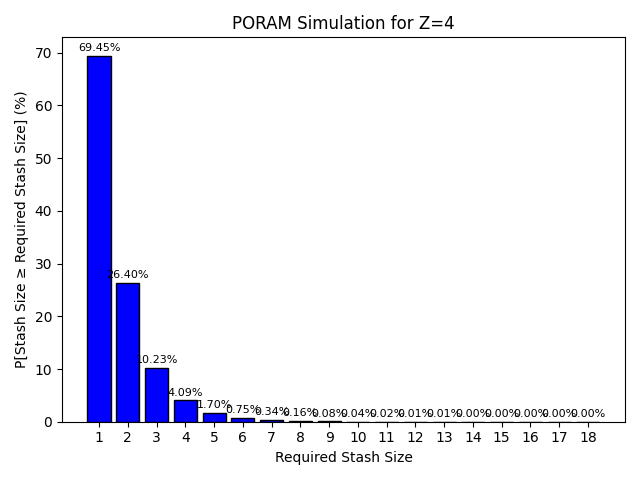
\includegraphics[width=\textwidth]{02-ex1/plot_z_2.png}
    \caption{Probabilty of stash overflow for $Z=2$.}
    \label{fig:stash-overflow-for-Z=2}
\end{figure}

\begin{figure}[H]
    \centering
    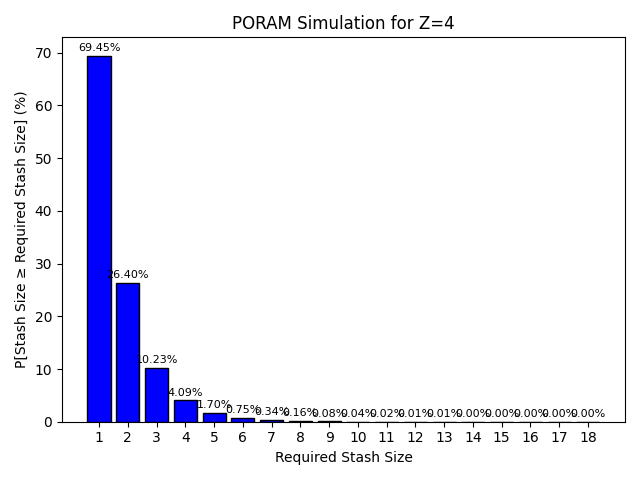
\includegraphics[width=\textwidth]{02-ex1/plot_z_4.png}
    \caption{Probabilty of stash overflow for $Z=4$.}
    \label{fig:stash-overflow-for-Z=4}
\end{figure}